% =============================================================================
% A criticality-anchored radius cannot escape a slow saddle in bounded time.
%
% Standalone. Own preamble, no bibliography, no \cite. The macro block mirrors
% the one near the top of _Thesis_FINAL/Article3/Survey-part3-v1.tex, through
% \providecommand, so this file can later be folded into that document.
% =============================================================================
\documentclass[11pt,a4paper]{article}

% \usepackage[T1]{fontenc}
\usepackage[utf8]{inputenc}
\usepackage[british]{babel}
\usepackage{amsmath, amssymb, amsthm}
\usepackage{booktabs}
\usepackage{graphicx}
\usepackage{geometry}
\usepackage{float}
\usepackage{enumitem}
\usepackage[hidelinks]{hyperref}
\geometry{margin=2.5cm}

% ---- macros mirrored from Survey-part3-v1.tex -------------------------------
\providecommand{\defeq}{\mathrel{:=}}
\providecommand{\kbar}{\overline{\kappa}}
\providecommand{\calO}{{\mathcal{O}}}
\providecommand{\calS}{{\mathcal{S}}}
\providecommand{\NN}{{\mathbb{N}}}
\providecommand{\abs}[1]{\left \vert #1 \right \vert}
\providecommand{\norm}[1]{\left \lVert #1 \right \rVert}
\providecommand*\mykappa[1]{ \kappa_{\scriptscriptstyle \text{#1}} }
\providecommand*\myeta[1]{ \eta_{\scriptscriptstyle \text{#1}} }
\providecommand{\Rdelta}{\textsf{R-delta}}
\providecommand{\Rstep}{\textsf{R-step}}
\providecommand{\Rdfo}{\textsf{R-DFO}}
\providecommand{\Rgrad}{\textsf{R-grad}}
\providecommand{\Rrtr}{\textsf{R-RTR}}
\providecommand{\Rgrtr}{\textsf{R-gRTR}}
\providecommand{\RAdaptiveGrad}{\textsf{R-adaptive-grad}}
\providecommand{\RAdaptstep}{\textsf{R-adaptive-step}}
\providecommand{\gone}{\gamma_1}
\providecommand{\gtwo}{\gamma_2}
\providecommand{\gthree}{\gamma_3}

\newtheorem{proposition}{Proposition}
\newtheorem{corollary}[proposition]{Corollary}
\newtheorem{lemma}[proposition]{Lemma}
\theoremstyle{definition}
\newtheorem{assumption}{Assumption}
\theoremstyle{remark}
\newtheorem{remark}{Remark}

\title{A criticality-anchored radius cannot escape a slow saddle\\ in bounded time}
\author{}
\date{}

\begin{document}
\maketitle

\begin{abstract}
A radius tied to a criticality measure inherits the measure's collapse near a
saddle. We prove a lower bound on the escape time that uses no property of the
model or of the subproblem solution beyond $\norm{s_k} \leq \Delta_k$, so the
stall survives perfect curvature information. For any cap $\overline{\mu}$ and
any $K$ there is an $\varepsilon$ giving escape time above $K$. We then measure
the constants. The fitted geometric rate agrees with the bound, the scaled
escape time collapses onto a single value across three decades of
$\overline{\mu}$ and five of $\varepsilon$, and the collapse constant is
$\ln(1/(\sqrt3\,y_0))$ rather than $\ln(1/(2y_0))$.
\end{abstract}

% =============================================================================
\section{The problem}\label{sec: problem}
% =============================================================================

For $\varepsilon > 0$ let
\begin{equation}
  f_\varepsilon(x,y) = \tfrac12 x^2
      + \varepsilon\left(\tfrac14 y^4 - \tfrac12 y^2\right) ,
  \qquad
  \nabla f_\varepsilon = \bigl(x,\ \varepsilon y(y^2-1)\bigr) .
  \label{eqn: f}
\end{equation}
The critical points are the origin and $(0,\pm1)$, with
\begin{equation}
  \nabla^2 f_\varepsilon(0,0) = \operatorname{diag}(1,-\varepsilon) ,
  \qquad
  \nabla^2 f_\varepsilon(0,\pm1) = \operatorname{diag}(1,2\varepsilon) .
  \label{eqn: hessians}
\end{equation}
The origin is a saddle, nonsingular for every $\varepsilon > 0$, so the
second-order measure reports $\tau(0,0) = \varepsilon$. The minimisers sit at
distance $1$ from the saddle whatever $\varepsilon$ is. So $\varepsilon$ tunes
the escape rate without moving the geometry.

\begin{lemma}[the line $\{x=0\}$ is invariant]\label{prop: invariant}
  Let $x_0 = 0$. Then $x_k = 0$ for every $k$, under truncated conjugate
  gradient and under the exact Mor\'e-Sorensen solver alike.
\end{lemma}

\begin{proof}
  At $x = 0$ the gradient is $(0, \varepsilon y(y^2-1))$, which lies along
  $e_2$, and the Hessian $\operatorname{diag}(1, \varepsilon(3y^2-1))$ is
  diagonal, so $He_2 \parallel e_2$. Conjugate gradient starts at $s = 0$ with
  residual $-g \parallel e_2$ and first direction $-g$. If $s_j \parallel e_2$
  and $d_j \parallel e_2$ then $Hd_j \parallel e_2$, the step length is a
  scalar, and $s_{j+1}$ and $d_{j+1}$ lie along $e_2$. Induction gives the
  claim. For the exact solver, $(H+\sigma I)^{-1}$ is diagonal, so
  $s^* = -(H+\sigma I)^{-1}g \parallel e_2$.
\end{proof}

Lemma~\ref{prop: invariant} was also checked numerically. Over the whole grid of
Section~\ref{sec: experiments}, $\max_k\abs{x_k}$ is $0$ in floating point, not
merely small.

On the invariant line, for $\abs{y} \leq 1$,
\begin{equation}
  \norm{g} = \varepsilon\abs{y}\,(1 - y^2) \leq \varepsilon\abs{y} .
  \label{eqn: gradient bound}
\end{equation}
The bound holds on $\abs{y} \leq 1$, not only on $\abs{y} \leq \tfrac12$.

% =============================================================================
\section{The proposition}\label{sec: proposition}
% =============================================================================

We state the hypothesis on the radius rule rather than on a named rule, so that
one statement covers both mechanisms.

\begin{assumption}[criticality-anchored radius]\label{as: RCA}
  There are $C > 0$ and $k_0 \geq 0$ such that
  \[
    \Delta_k \;\leq\; C \max_{k_0 \leq j \leq k} \norm{g_j}
    \qquad\text{for all } k \geq k_0 .
  \]
\end{assumption}

The running maximum is what makes the assumption cover $\Rdfo$, whose radius is
controlled by $\norm{g_{k-1}}$ rather than by $\norm{g_k}$. Nothing else in the
proof needs it.

\begin{proposition}[escape time]\label{prop: escape}
  Let $x_0 = 0$ and $0 < \abs{y_{k_0}} \leq \tfrac12$. Suppose the run satisfies
  Assumption~\ref{as: RCA} with constants $C$ and $k_0$. Write
  \[
    k_{\mathrm{esc}} = \min\{k : \abs{y_k} > \tfrac12\} .
  \]
  Then
  \begin{equation}
    k_{\mathrm{esc}} \;>\; k_0
      + \frac{\ln\bigl(1/(2\abs{y_{k_0}})\bigr)}{\ln(1 + C\varepsilon)} .
    \label{eqn: escape}
  \end{equation}
\end{proposition}

\begin{proof}
  Write $M_k = \max_{k_0 \leq j \leq k}\abs{y_j}$. Every trust-region step
  satisfies $\norm{s_k} \leq \Delta_k$, and by Lemma~\ref{prop: invariant} the
  step lies along $e_2$, so
  \[
    \abs{y_{k+1}} \leq \abs{y_k} + \norm{s_k} \leq \abs{y_k} + \Delta_k .
  \]
  The inequality also covers a rejected step, for which $y_{k+1} = y_k$.

  Let $k_0 \leq k < k_{\mathrm{esc}}$. Then $\abs{y_j} \leq \tfrac12$ for every
  $j \leq k$, so \eqref{eqn: gradient bound} applies at each such $j$ and gives
  $\norm{g_j} \leq \varepsilon\abs{y_j} \leq \varepsilon M_k$. With
  Assumption~\ref{as: RCA},
  \[
    \Delta_k \leq C \max_{k_0 \leq j \leq k}\norm{g_j} \leq C\varepsilon M_k ,
  \]
  hence $\abs{y_{k+1}} \leq M_k(1 + C\varepsilon)$. Since $1 + C\varepsilon > 1$,
  \[
    M_{k+1} = \max\{M_k, \abs{y_{k+1}}\} \leq M_k(1 + C\varepsilon) ,
  \]
  and by induction $M_k \leq \abs{y_{k_0}}(1+C\varepsilon)^{k-k_0}$.

  At $k = k_{\mathrm{esc}}$ we have $\abs{y_{k}} > \tfrac12$, so
  $M_{k_{\mathrm{esc}}} > \tfrac12$ and
  $\abs{y_{k_0}}(1+C\varepsilon)^{k_{\mathrm{esc}}-k_0} > \tfrac12$. Taking
  logarithms gives \eqref{eqn: escape}.
\end{proof}

\begin{remark}
  The proof uses no property of the model or of the subproblem solution beyond
  $\norm{s_k} \leq \Delta_k$. That is what makes it a statement about the radius
  axis. In particular it holds with the exact Hessian, and the experiments of
  Section~\ref{sec: experiments} use the exact Hessian throughout.
\end{remark}

\begin{corollary}[an $\varepsilon$ for every budget]\label{prop: budget}
  Fix $\overline{\mu} > 0$, $0 < \abs{y_0} < \tfrac12$ and $K > 0$. If
  \[
    0 < \varepsilon < \frac{\ln\bigl(1/(2\abs{y_0})\bigr)}{\overline{\mu}K} ,
  \]
  then any run satisfying Assumption~\ref{as: RCA} with $C = \overline{\mu}$ and
  $k_0 = 0$ has $k_{\mathrm{esc}} > K$.
\end{corollary}

\begin{proof}
  The hypothesis gives
  $\overline{\mu}\varepsilon < \ln(1/(2\abs{y_0}))/K$, and $\ln(1+t) < t$ for
  $t > 0$, so $\ln(1+\overline{\mu}\varepsilon) < \ln(1/(2\abs{y_0}))/K$.
  Substituting into \eqref{eqn: escape} gives $k_{\mathrm{esc}} > K$.
\end{proof}

\subsection{The two mechanisms}\label{sec: mechanisms}

$\Rgrad(\omega,\overline{\mu})$ sets $\Delta_k = \mu_k\norm{g_k}$ with
$\mu_k \leq \overline{\mu}$, so Assumption~\ref{as: RCA} holds with
$C = \overline{\mu}$ and $k_0 = 0$. This is immediate and needs no entry
condition.

$\Rdfo(\omega)$ is different, and the difference is not cosmetic. Its update is
\begin{equation}
  \Delta_{k+1} =
  \begin{cases}
    \gone\Delta_k, & \rho_k < \eta_1, \\
    \gtwo\Delta_k, & \rho_k \geq \eta_1 \text{ and } \Delta_k > \zeta\norm{g_k}, \\
    \gthree\Delta_k, & \rho_k \geq \eta_1 \text{ and } \Delta_k \leq \zeta\norm{g_k},
  \end{cases}
  \label{eqn: rdfo}
\end{equation}
so the radius is tied to the criticality measure only inside the band
$\Delta_k \leq \zeta\norm{g_k}$.

\begin{proposition}[the \textnormal{$\Rdfo$} version, with its entry condition]
\label{prop: rdfo}
  Suppose there is $k_0$ with $\Delta_{k_0} \leq \zeta\norm{g_{k_0}}$. Then
  Assumption~\ref{as: RCA} holds for $k > k_0$ with $C = \gthree\zeta$, and
  \eqref{eqn: escape} applies with that constant.

  If no such $k_0$ exists, then $\Delta_k \to 0$ geometrically,
  $\norm{g_k} \to 0$, and on the invariant line $\abs{y_k} \to 0$. The run
  converges to the saddle and never escapes.
\end{proposition}

\begin{proof}
  Write $S_k = \max_{k_0 \leq j \leq k}\norm{g_j}$. At $k_0$ the hypothesis gives
  $\Delta_{k_0} \leq \zeta\norm{g_{k_0}} \leq \gthree\zeta S_{k_0}$, since
  $\gthree > 1$. Suppose $\Delta_k \leq \gthree\zeta S_k$. If
  $\Delta_k \leq \zeta\norm{g_k}$, then \eqref{eqn: rdfo} gives
  $\Delta_{k+1} \leq \gthree\Delta_k \leq \gthree\zeta\norm{g_k} \leq
  \gthree\zeta S_k$. Otherwise $\Delta_{k+1} \leq \max\{\gone,\gtwo\}\Delta_k
  < \Delta_k \leq \gthree\zeta S_k$. Either way
  $\Delta_{k+1} \leq \gthree\zeta S_k \leq \gthree\zeta S_{k+1}$, which is
  Assumption~\ref{as: RCA} with $C = \gthree\zeta$.

  For the second statement, if $\Delta_k > \zeta\norm{g_k}$ for every $k$, then
  both remaining branches of \eqref{eqn: rdfo} contract, so
  $\Delta_k \leq \max\{\gone,\gtwo\}^{\,k}\Delta_0 \to 0$. Then
  $\norm{g_k} < \Delta_k/\zeta \to 0$. On the invariant line
  $\norm{g_k} = \varepsilon\abs{y_k}(1-y_k^2)$ with $1 - y_k^2 \geq \tfrac34$
  below the threshold, so $\abs{y_k} \to 0$.
\end{proof}

\begin{remark}
  The entry condition bites. Started at $\Delta_0 = 1$ from $y_0 = 10^{-3}$ with
  $\varepsilon = 10^{-3}$, the run has $\Delta_0/\norm{g_0} \approx 10^{6}$, far
  outside the band, and it escapes at $k = 1$ for every $\zeta$ and every
  $\varepsilon$ in the grid. Proposition~\ref{prop: rdfo} says nothing about such
  a run, and it should not. Section~\ref{sec: experiments} therefore reports a
  separate arm started at $\Delta_0 = \zeta\norm{g_0}$, which satisfies the entry
  condition at $k_0 = 0$ by construction.
\end{remark}

\subsection{Relation to Part~II}\label{sec: partII}

Part~II already contains the qualitative statement. Its
\texttt{cond: s\_k bounded by g\_k}, labelled C.Sg, requires
$\norm{s_k} \leq \kbar\norm{g_k}$ near $x^*$ from some index on.
\texttt{thm: convergence to potential saddle point} shows that a subsequence
converging to a nonsingular first-order critical point, together with C.Sg,
forces the whole sequence to converge there.
\texttt{cor: convergence criticality anchored saddle} then states that
$\{x_k\}$ converges to $x^*$ if the mechanism is $\Rgrad$ with
$\mu_k \leq \overline{\mu}$, or if it is $\Rdfo$.

Proposition~\ref{prop: escape} is the quantitative complement. Part~II says the
criticality-anchored rules cannot leave the saddle asymptotically. This says how
slowly they fail to leave it, and Corollary~\ref{prop: budget} converts that into
a budget.

Two differences are worth recording. Part~II's prose states that $\Rdfo$ does not
satisfy C.Sg and reaches the same conclusion by another route.
Assumption~\ref{as: RCA} is stated on $\Delta_k$ with a running maximum, and
covers both rules for that reason. The induction of
Proposition~\ref{prop: rdfo} is a relaxation of the bound inside the proof of
\texttt{cor: convergence criticality anchored saddle}, which carries an
additional $\gtwo^{\,k-k^--1}$ factor and is therefore sharper.

Part~II also states the repair that Section~\ref{sec: measures} measures. Near a
saddle $\norm{g_k} \to 0$ while $-\lambda^-_k$ stays bounded away from zero, so
$\tau_k$ inherits a floor, and Part~II records that it is
\texttt{thm: second-order convergence}, not the mechanism, that converts the
floor into escape.

% =============================================================================
\section{Experiments}\label{sec: experiments}
% =============================================================================

The grid takes $\varepsilon$ over five decades from $10^{-1}$ to $10^{-5}$,
$\overline{\mu}$ and $\zeta$ over three decades, $y_0 \in \{10^{-3},10^{-6}\}$
and $x_0 \in \{0, 0.8\}$. The model is the true Hessian and the subproblem
solver is truncated conjugate gradient throughout, so the stall appears with
perfect curvature information. $\Rdelta$ runs from the same starting points as
the comparator.

Two tolerances are used and never pooled. The rate regime takes
$\texttt{tol} = 10^{-14}$, which lets the dynamics run so that
$k_{\mathrm{esc}}$ and the fitted rate are measurable. The outcome regime takes
$\texttt{tol} = 10^{-5}$, which is where false convergence appears. A run that
has not escaped within $50\,000$ iterations is reported \texttt{never} and is
never treated as a number.

\subsection{The radius is the binding quantity}

Across the $\Rgrad$ grid the median $\theta_k = \Delta_k/\norm{g_k}$ equals
$\overline{\mu}$ to six figures, and the trust-region constraint is active on
every iteration of almost every cell. The radius is therefore what limits the
step, rather than the subproblem solution.

\subsection{The fitted rate}\label{sec: rate}

The escape phase is defined by $\abs{x_k} \leq \varepsilon\abs{y_k}$ and
$\abs{y_k} \leq \tfrac12$. On the $x_0 = 0$ arm the first condition is vacuous
and the phase is the whole pre-escape run. Regressing $\log\abs{y_k}$ on $k$ over
that phase gives the fitted rate.

The fitted rate tracks $\ln(1+\overline{\mu}\varepsilon)$ closely and from below,
which is the side Proposition~\ref{prop: escape} predicts, since the proposition
bounds growth from above. At $\overline{\mu}\varepsilon = 10^{-3}$ the fitted
rate is $0.00099$ against $0.00100$; at $10^{-2}$ it is $0.00986$ against
$0.00995$; at $10^{-1}$ it is $0.09454$ against $0.09531$. The one cell with
$\overline{\mu}\varepsilon = 1$ gives $0.58752$ against $0.69315$, where the
linearisation no longer applies. Figure~\ref{fig: rate} plots the comparison.

\subsection{The collapse, and its constant}\label{sec: collapse}

The scaled escape time $\overline{\mu}\varepsilon k_{\mathrm{esc}}$ collapses
onto one value across three decades of $\overline{\mu}$ and five of
$\varepsilon$. The measured value is $6.362$ at $y_0 = 10^{-3}$ and $13.273$ at
$y_0 = 10^{-6}$.

The predicted constant $\ln(1/(2y_0))$ is $6.215$ and $13.122$, leaving
residuals of $0.147$ and $0.151$. The continuous limit of the recursion is
$\mathrm{d}y/\mathrm{d}k = C\varepsilon y(1-y^2)$, whose integral from $y_0$ to
$\tfrac12$ is
\begin{equation}
  \int_{y_0}^{1/2}\frac{\mathrm{d}y}{y(1-y^2)}
  = \ln\frac{1}{\sqrt3\,y_0} + \calO(y_0^2) .
  \label{eqn: exact constant}
\end{equation}
That gives $6.3585$ and $13.2663$, leaving residuals of $0.0035$ and $0.0067$,
smaller by a factor of about forty. The $\sqrt3$ comes from the factor $1-y^2$ at
the escape threshold, not from the threshold itself.

\subsection{The two criticality measures}\label{sec: measures}

With $\omega_k = \tau_k$ the radius near the saddle is about
$\overline{\mu}\varepsilon$, a constant rather than a quantity proportional to
$\abs{y_k}$, so growth becomes arithmetic. The ratio of the two escape times is
measured at $8.64$, and it is stable across the grid: the individual cells give
$8.635$, $8.644$, $8.644$ and $9.571$, with no trend in $\varepsilon$ or in
$\overline{\mu}$. The structural prediction, that the ratio does not depend on
$\varepsilon$, therefore holds.

The predicted value $2\ln(1/(2y_0)) = 12.43$ does not. Repeating
\eqref{eqn: exact constant} for $\tau = \varepsilon(1-3y^2)$ gives
\[
  \int_{y_0}^{1/2}\frac{\mathrm{d}y}{1-3y^2}
  = \frac{\operatorname{artanh}(\sqrt3/2)}{\sqrt3} + \calO(y_0)
  = 0.7604 ,
\]
so the ratio should be $6.3585/0.7604 = 8.362$, within three per cent of what is
measured. The arithmetic prediction $k_{\mathrm{esc}} \approx 1/(2\overline{\mu}
\varepsilon)$ omits the decrease of $\tau_k$ as $\abs{y_k}$ grows, which is what
the factor $0.7604$ against $0.5$ records.

The extra curvature is not free. At $\overline{\mu} = 1$ and
$\varepsilon = 10^{-2}$ the $\norm{g}$-anchored run uses $1502$
Hessian-vector products and the $\tau$-anchored run $940$, so on that cell the
second measure is cheaper in total because it escapes sooner, while costing more
per iteration.

\subsection{Three outcomes}\label{sec: outcomes}

At $\texttt{tol} = 10^{-5}$, $136$ of the $160$ $\Rgrad$ and $\Rdfo$ cells end in
false convergence, against $12$ fast escapes, $11$ slow and $1$ that never
escapes. Rerunning those $136$ cells with the second-order stopping test at
$\texttt{tol\_H} = 10^{-6}$ leaves none of them false-convergent: $68$ become
fast escapes, $29$ slow, and $39$ do not escape within the budget. A method that
refuses to stop at the saddle escapes slowly instead, and in $39$ cells the wrong
answer becomes one that does not finish.

The radius measure and the stopping test are two different uses of second-order
information and are reported separately throughout.

\subsection{The \textnormal{$\Rdfo$} arm}

Started at $\Delta_0 = \zeta\norm{g_0}$, so that the entry condition holds at
$k_0 = 0$, the $\Rdfo$ runs stall exactly as the proposition requires. The
measured $\theta_k$ settles at $\zeta$ rather than at $\gthree\zeta$, and the
fitted rate is correspondingly about half the bound: at $\zeta\varepsilon =
10^{-3}$ the fitted rate is $0.00103$ against the bound $\ln(1+\gthree\zeta
\varepsilon) = 0.00200$. The bound of Proposition~\ref{prop: rdfo} therefore
holds and is not tight, the factor $\gthree$ being the worst case of an
expansion that the next iteration undoes. Scaling by $\zeta$ rather than by
$\gthree\zeta$ puts the collapse at $6.048$, near the $\Rgrad$ value.

\begin{figure}[H]\centering
  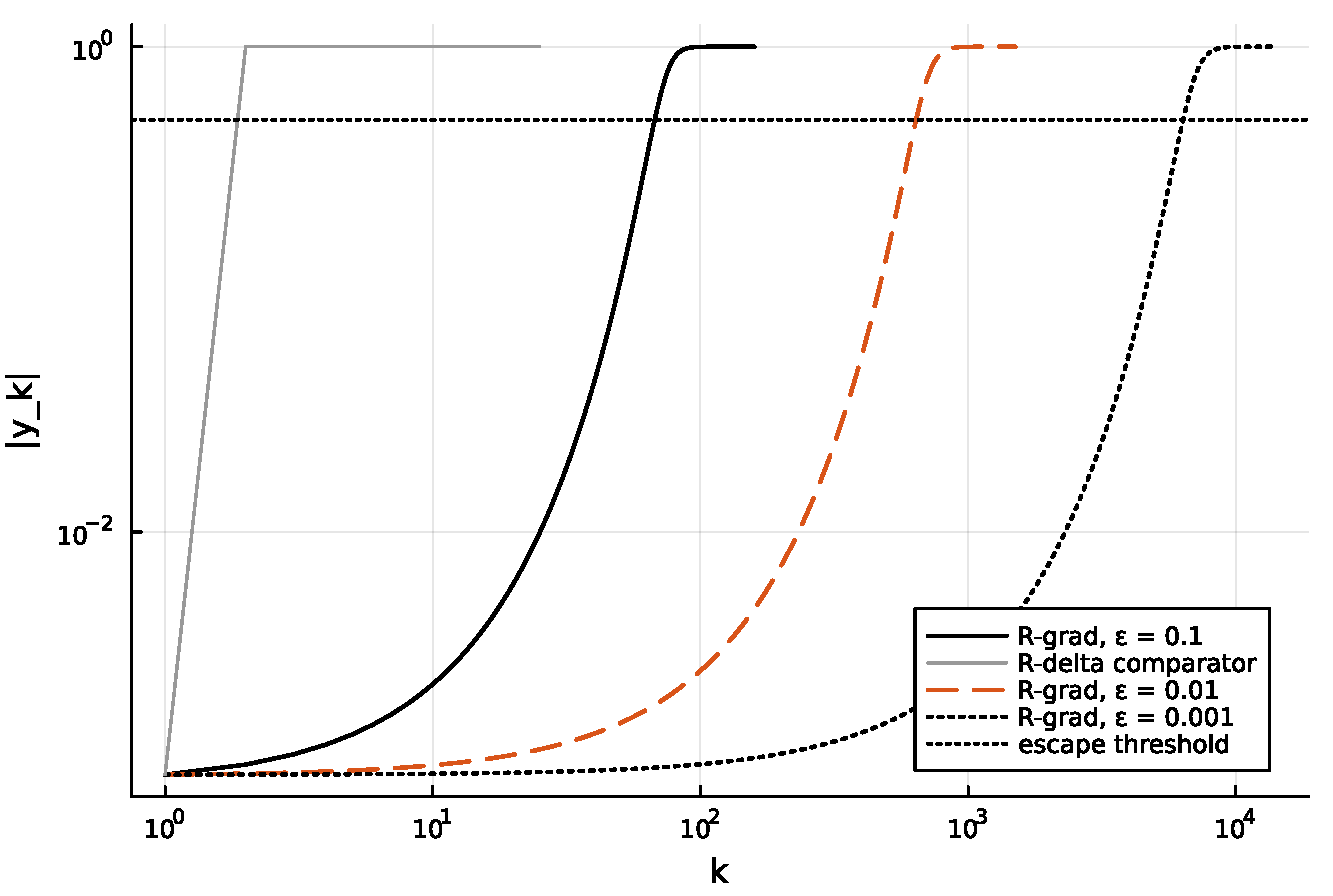
\includegraphics[width=0.66\textwidth]{figs/exp15_fig1_y_vs_k.pdf}
  \caption{$\abs{y_k}$ against $k$ for three values of $\varepsilon$ at
  $\overline{\mu} = 1$, with the $\Rdelta$ comparator in grey and the escape
  threshold dotted.}
  \label{fig: trajectories}
\end{figure}

\begin{figure}[H]\centering
  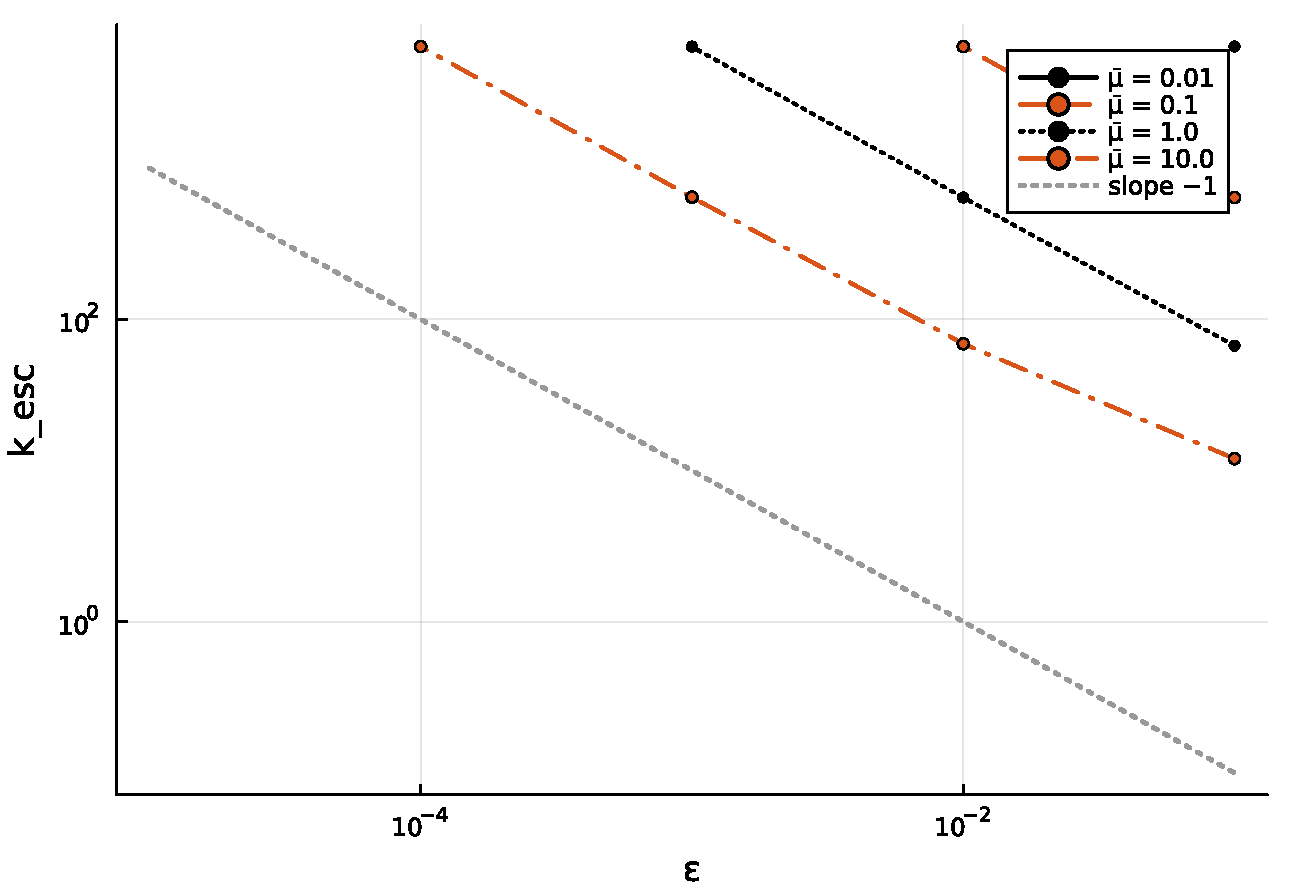
\includegraphics[width=0.66\textwidth]{figs/exp15_fig2_kesc_vs_eps.pdf}
  \caption{$k_{\mathrm{esc}}$ against $\varepsilon$, one series per
  $\overline{\mu}$, with the predicted slope $-1$.}
  \label{fig: kesc}
\end{figure}

\begin{figure}[H]\centering
  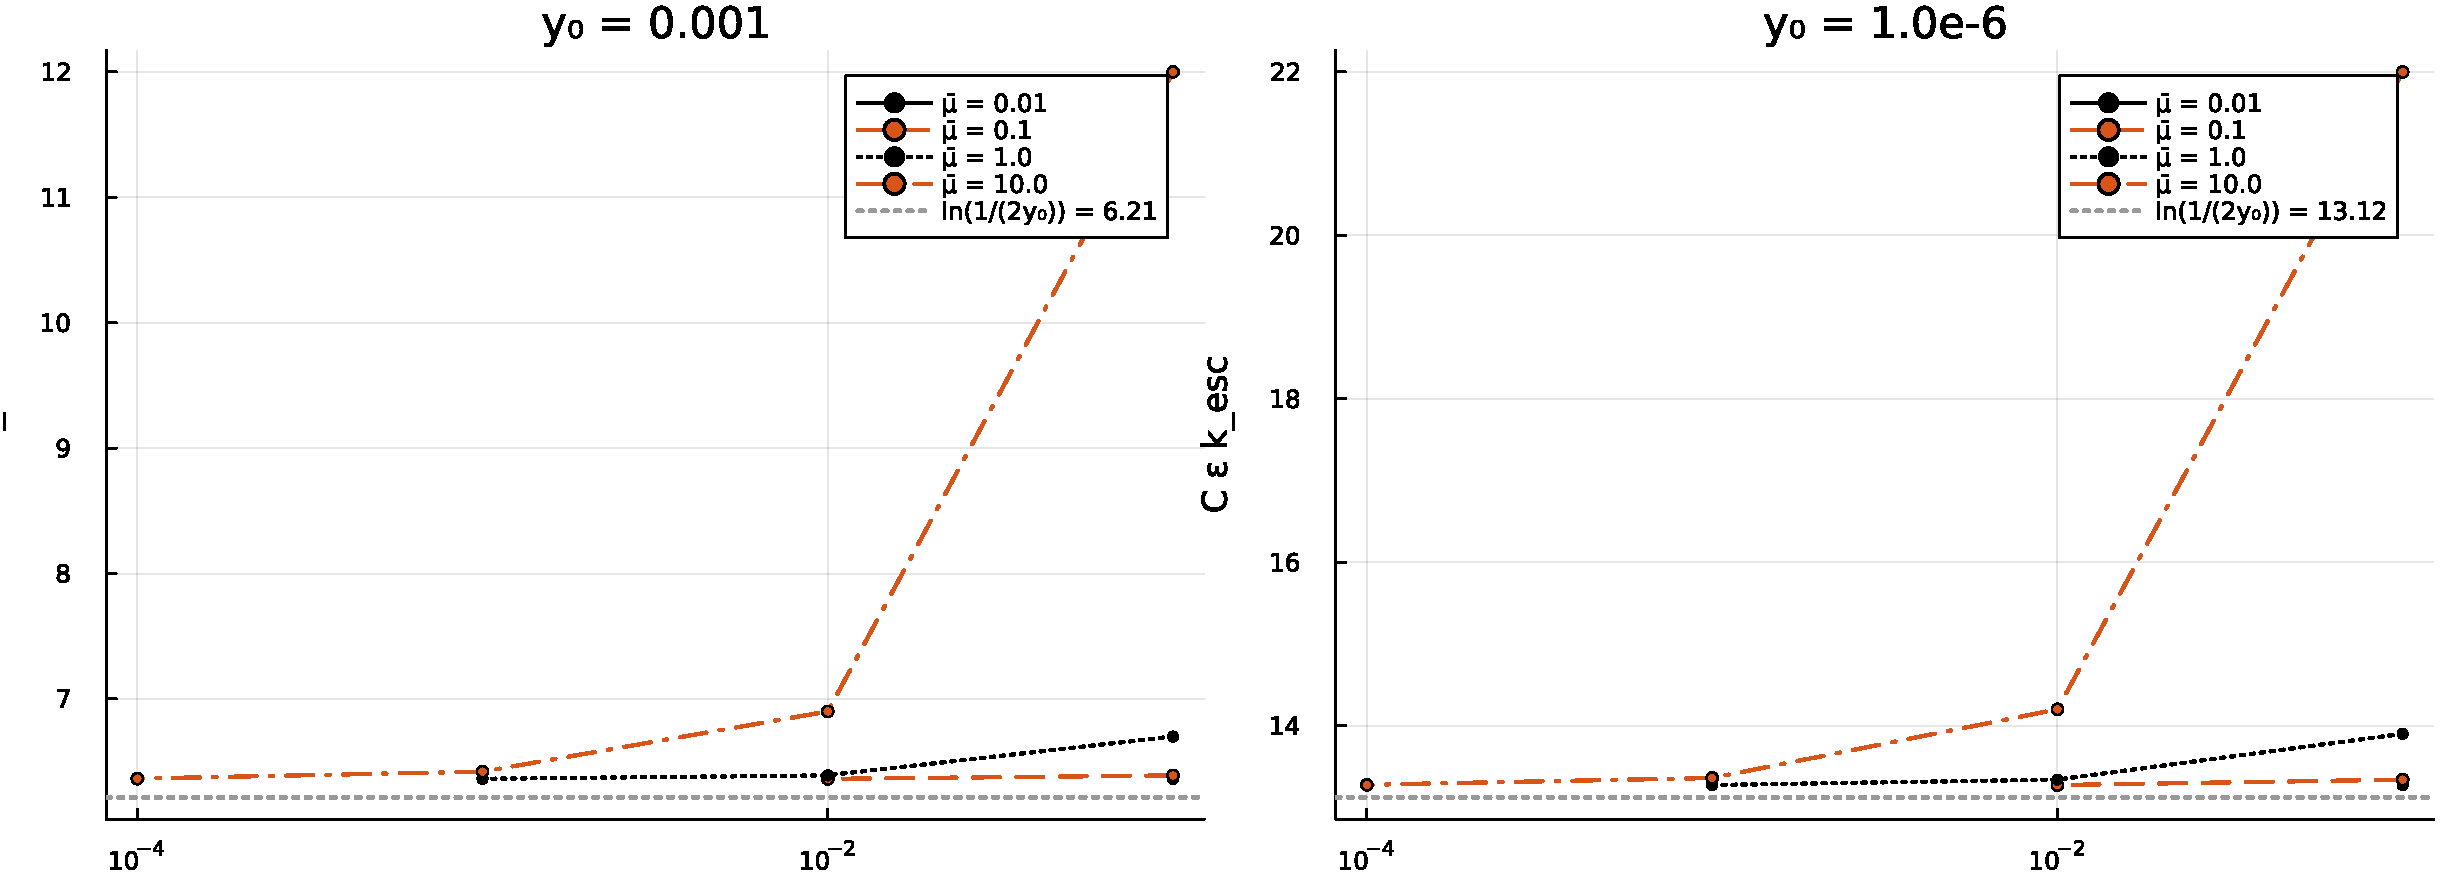
\includegraphics[width=\textwidth]{figs/exp15_fig3_collapse.pdf}
  \caption{The collapse. $\overline{\mu}\varepsilon k_{\mathrm{esc}}$ against
  $\varepsilon$ for the whole grid, one panel per $y_0$, with
  $\ln(1/(2y_0))$ marked.}
  \label{fig: collapse}
\end{figure}

\begin{figure}[H]\centering
  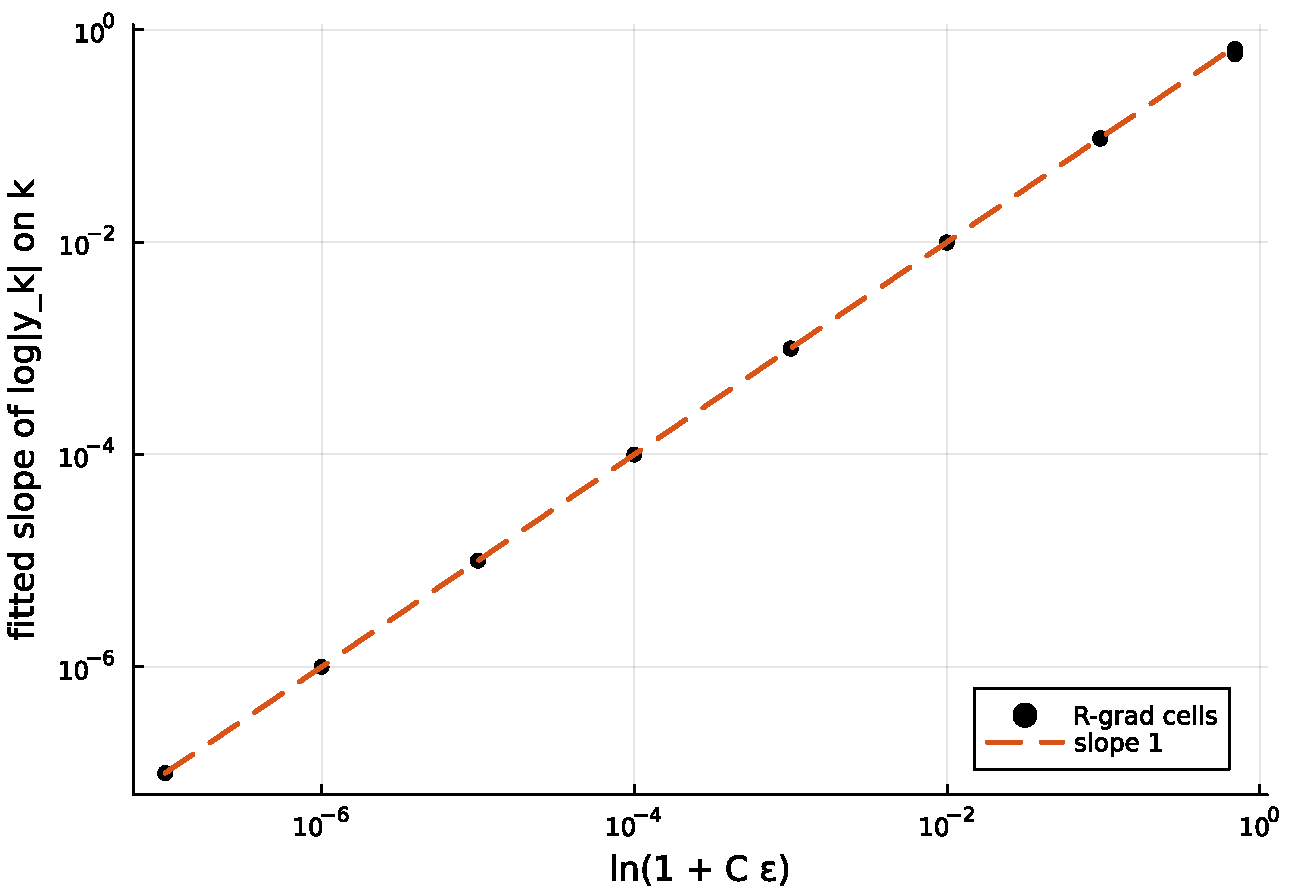
\includegraphics[width=0.66\textwidth]{figs/exp15_fig4_rate.pdf}
  \caption{The fitted geometric rate against $\ln(1+\overline{\mu}\varepsilon)$,
  with the line of slope $1$.}
  \label{fig: rate}
\end{figure}

\begin{figure}[H]\centering
  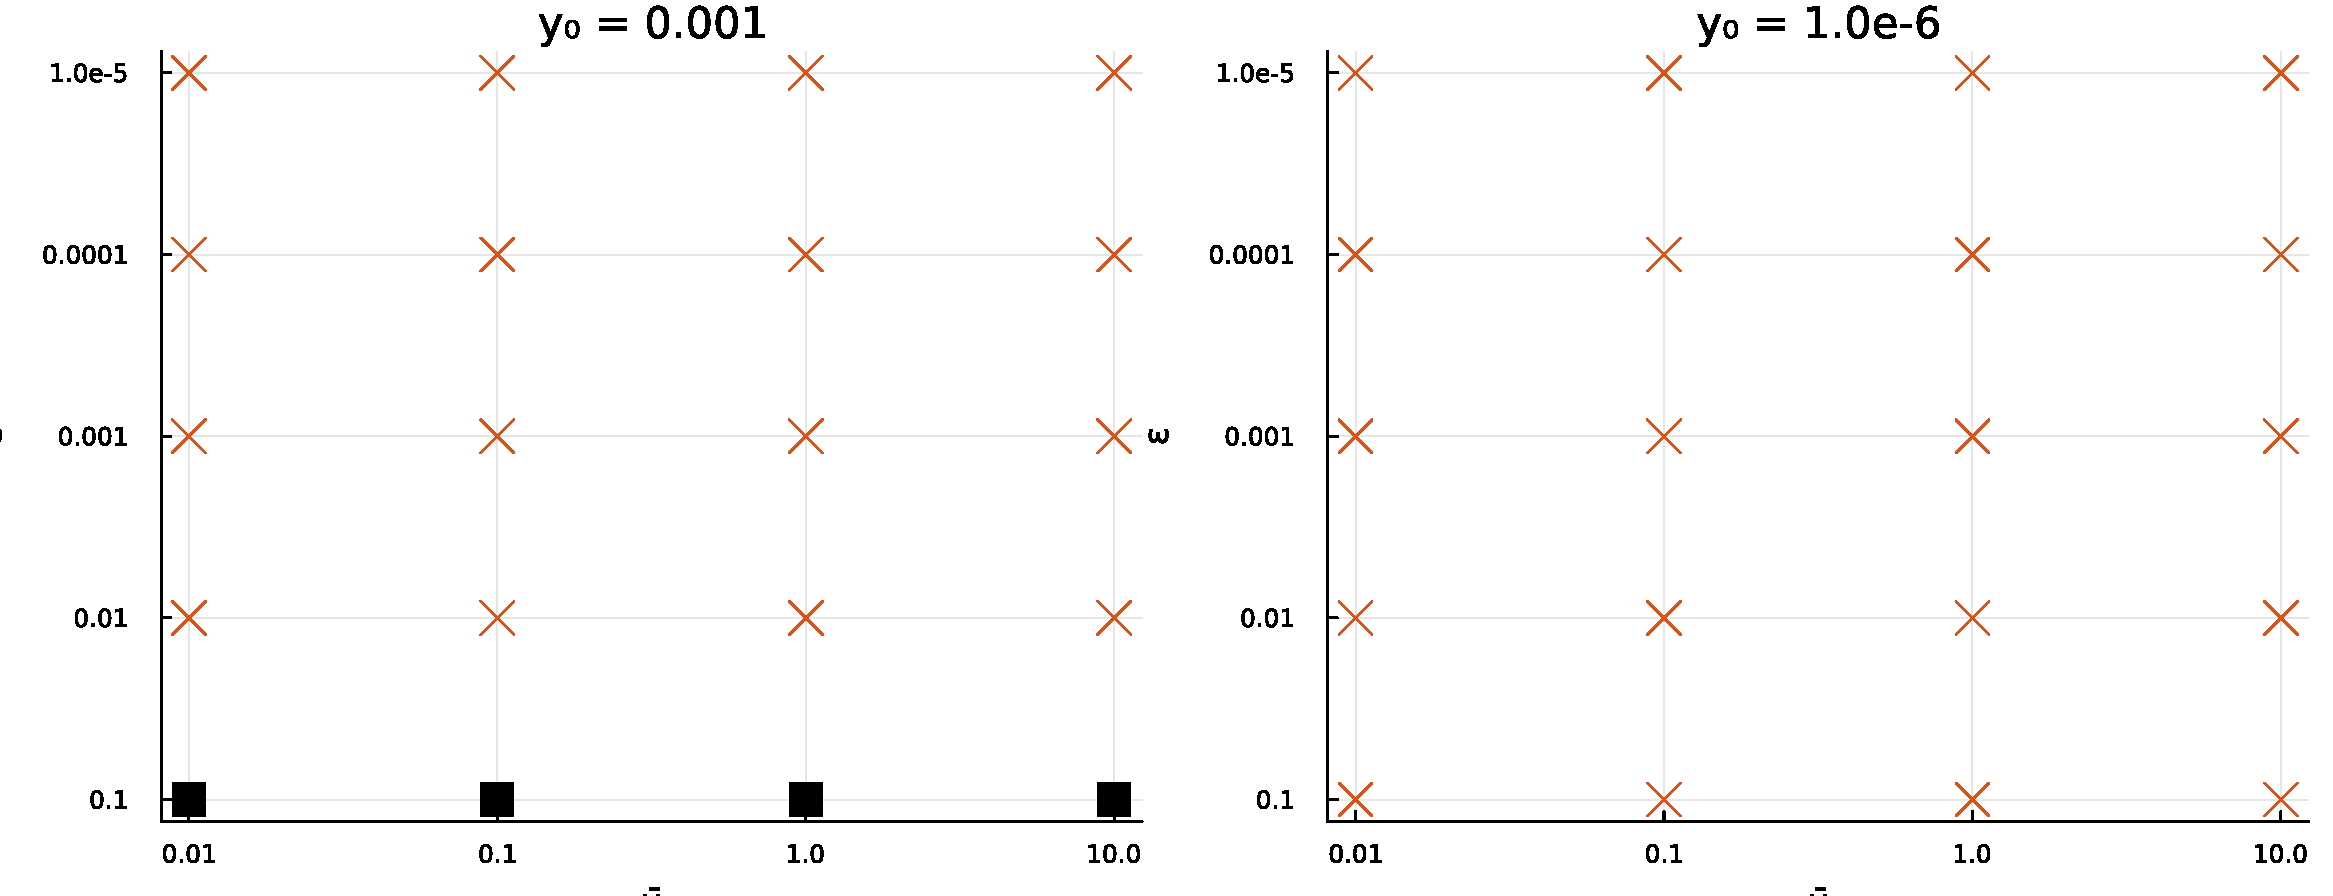
\includegraphics[width=\textwidth]{figs/exp15_fig5_outcomes.pdf}
  \caption{The three outcomes over the $(\overline{\mu},\varepsilon)$ grid at
  first-order tolerance $10^{-5}$, which is the tolerance that draws the
  boundary. Crosses mark false convergence, circles fast escape, squares slow
  escape or none.}
  \label{fig: outcomes}
\end{figure}

\begin{figure}[H]\centering
  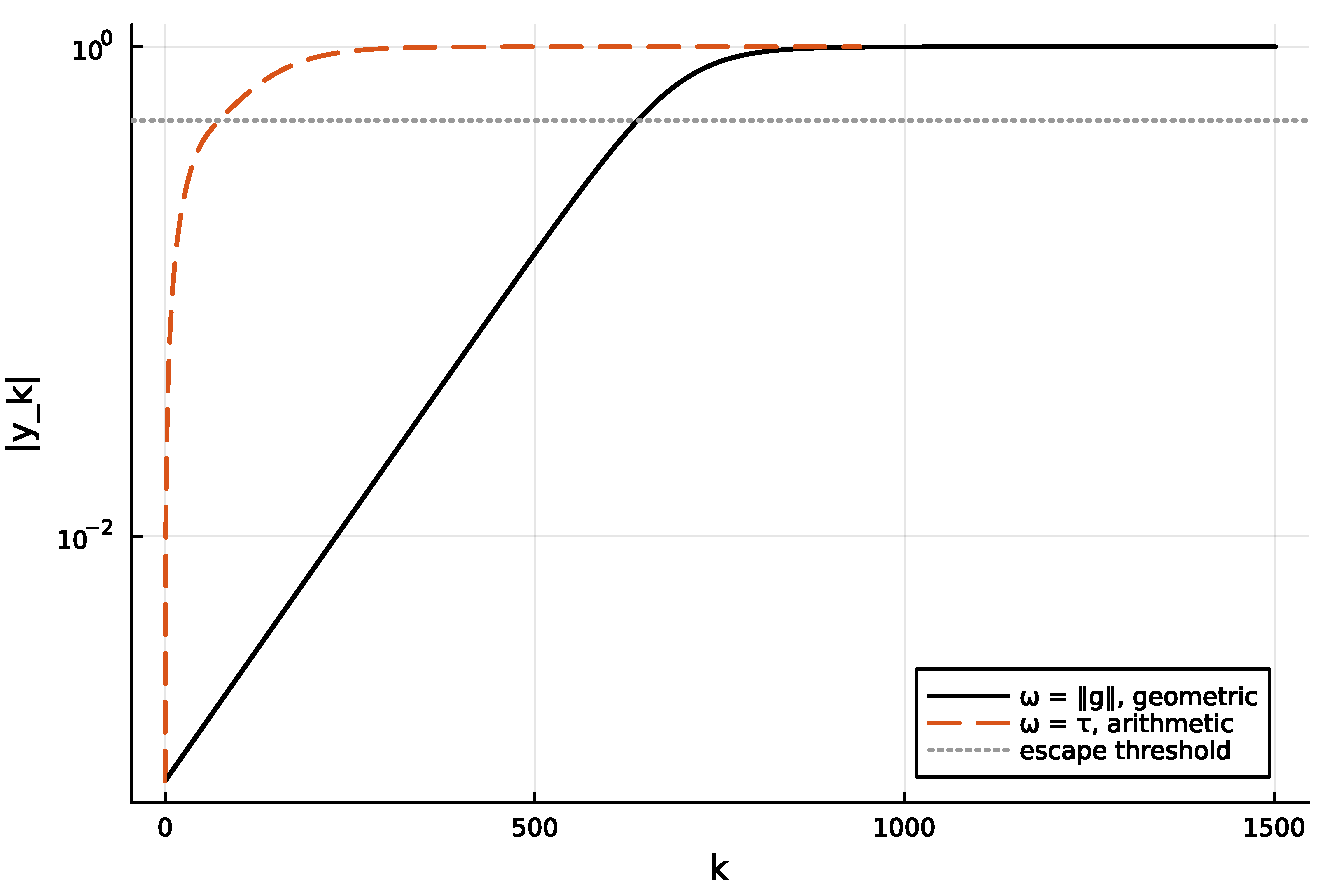
\includegraphics[width=0.66\textwidth]{figs/exp15_fig6_measures.pdf}
  \caption{$\omega_k = \norm{g_k}$ against $\omega_k = \tau_k$ at
  $\overline{\mu} = 1$, $\varepsilon = 10^{-2}$, $y_0 = 10^{-3}$. Geometric
  growth against arithmetic growth.}
  \label{fig: measures}
\end{figure}

% =============================================================================
\section{Findings for the existing subsection}\label{sec: findings}
% =============================================================================

These are proposals. We did not edit the source. Line numbers are from
\texttt{\_Thesis\_FINAL/Article3/Survey-part3-v1.tex}.

\begin{enumerate}[leftmargin=2em]
  \item \textbf{Line 1109, a self-reference.} The caption ends
        \texttt{This table isolates the model axis; Section\textasciitilde
        \textbackslash ref\{subsec: flat\} adds the radius axis.} The table sits
        inside the subsection carrying \texttt{\textbackslash label\{subsec:
        flat\}} at line 1051, so the cross-reference points at its own section.

  \item \textbf{Line 1096, a false statement.} The source reads
        \texttt{\$\textbackslash norm\{g\_0\} \textbackslash approx
        \textbackslash varepsilon y\_0 = 10\^{}\{-10\}\$}. With
        $x_0 = (0.8, y_0)$ the measured $\norm{g_0}$ is $0.800000$, larger by a
        factor of $8\times10^{9}$. A sentence that says what happens without
        changing the claim: \emph{the $x$ component is solved first, after which
        $\norm{g_k}$ falls to $\varepsilon\abs{y_0} = 10^{-10}$ and the method
        meets its stopping criterion at a nonsingular saddle.} The number of
        iterations depends on $\Delta_0$, which the caption does not state.
        Under $\Delta_0 = 1$ the drop happens in one iteration.

  \item \textbf{Line 1107, the invariant.} The caption says
        $\varepsilon k_{\mathrm{esc}}$ is constant at $\approx \ln(1/y_0)$. Over
        the seven printed rows with a $k_{\mathrm{esc}}$, the mean absolute
        residual is $0.4304$ for $\ln(1/y_0)$, $0.3155$ for $\ln(1/(2y_0))$ and
        $0.1716$ for $\ln(1/(\sqrt3\,y_0))$. Restricted to the rows with
        $\varepsilon \leq 10^{-3}$, where the continuous limit applies, the
        residuals for $\ln(1/(\sqrt3\,y_0))$ are $0.0036$, $0.0068$ and
        $0.0004$. The $\tfrac12$ improves the fit, and $\sqrt3$ improves it
        further, for the reason given at \eqref{eqn: exact constant}.

  \item \textbf{Line 1125, an em dash.} The last row contains a
        \texttt{-{}-{}-} cell, which sets an em dash. Leave it empty or mark it
        \texttt{n/a}.

  \item \textbf{The status column.} \texttt{stagnated} and \texttt{converged}
        record two different events. \texttt{converged} means
        $\norm{g_k} \leq 10^{-9}$, a mathematical criterion.
        \texttt{stagnated} means the achieved reduction fell to the rounding
        level of $f$ with a numerically nil step, an arithmetic event that says
        the run stopped making progress rather than that it found anything. The
        column should say which.
\end{enumerate}

% =============================================================================
\section{Where this belongs}\label{sec: home}
% =============================================================================

Proposition~\ref{prop: escape} and Corollary~\ref{prop: budget} are candidates
for the subsection of Part~II carrying \texttt{subsec:Danger of saddle points},
immediately after
\texttt{cor: convergence criticality anchored saddle}, which they quantify. The
experimental sections are candidates for the subsection of the numerical study
carrying \texttt{subsec: flat}, whose own note asks for the
$(\overline{\mu},\varepsilon)$ grid with the $\Rdelta$ comparator.

\end{document}
